\chapter{РАБОТА С КОМАНДНОЙ ОБОЛОЧКОЙ BASH}

\section{Цель работы}
Изучить базовые операции в терминале bash: навигацию по файловой системе, чтение файлов, создание и удаление директорий и файлов, работу с ключами и аргументами команд, а также создание/извлечение архивов с помощью tar. Зафиксировать историю команд в файле \texttt{record\_result}.

\section{Краткий ход выполнения}

\subsection{Подготовка и запуск записи команд}
\begin{enumerate}
  \item Запуск терминала и включение записи команд: \texttt{script -a record\_result}
  \item Проверка наличия файла записи: \texttt{ls -l}
\end{enumerate}

\subsection{Навигация и генерация варианта}
\begin{enumerate}
  \item Переход на рабочий стол: \texttt{cd ~/Desktop} (либо \texttt{cd ~/Рабочий\textbackslash{} стол/})
  \item Проверка наличия \texttt{lab2.py}: \texttt{ls -l}
  \item Генерация задания и фиксирование результата (скриншот): \texttt{python lab2.py}
\end{enumerate}

\subsection{Исследование структуры и просмотр содержимого файлов}
\begin{enumerate}
  \item Переход по дереву директорий: \texttt{cd}, \texttt{ls -l}, \texttt{pwd}, \texttt{cd ..}, \texttt{cd ./relative/path}
  \item Поиск текстового файла и вывод содержимого: \texttt{cat имя\_файла} (фрагмент добавить в отчет)
  \item Рисунок-«дерево» структуры директории (вставить в отчет)
\end{enumerate}

\subsection{Манипулирование файлами}
\begin{enumerate}
  \item Создание структуры каталогов по \texttt{Task 2}: \texttt{mkdir -p}
  \item Создание файлов: \texttt{touch фамилия\_1 фамилия\_2 фамилия\_3}
  \item Редактирование в \texttt{nano}: \texttt{nano file\_name}
  \item Копирование: \texttt{cp фамилия\_1 copy\_name}
  \item Перемещение и переименование: \texttt{mv фамилия\_2 ./dir\_name/new\_name\_2}
  \item Удаление: \texttt{rm -rf фамилия\_3}
  \item Массовое удаление по шаблону: \texttt{find . -type f -name '*[0-9]' -delete}
\end{enumerate}

\subsection{Ключи и аргументы команд tar}
\begin{itemize}
  \item Создание архива: ключ \texttt{-c}
  \item Извлечение архива: ключ \texttt{-x}
  \item Выбор компрессии: ключ \texttt{-z} (gzip), \texttt{-j} (bzip2), \texttt{-J} (xz)
  \item Имя файла архива: ключ \texttt{-f}
\end{itemize}
Создание архива: \texttt{tar -czf my\_new\_archive.tar.gz ./root\_dir}

Извлечение и чтение секрета из \texttt{Task 3}: \texttt{tar -xzf task3\_archive.tar.gz}, затем \texttt{cat ./path/to/secret\_file}

\section{Скриншоты (шаблоны вставки)}


\begin{figure}[H]
  \centering
  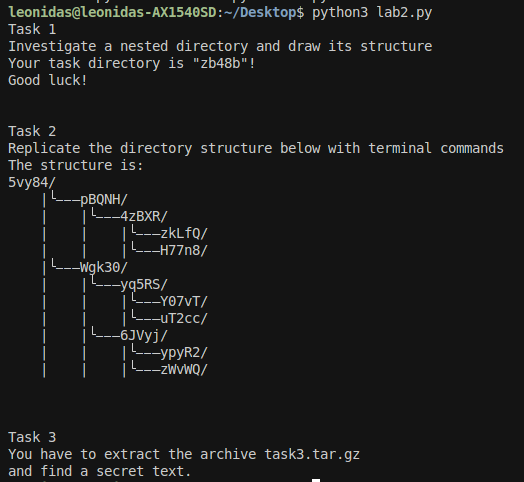
\includegraphics[width=0.95\textwidth]{images/image.png}
  \caption{Дерево файлов из генерации заданий (Task 2)}
  \label{fig:gen_tree}
\end{figure}

\begin{figure}[H]
  \centering
  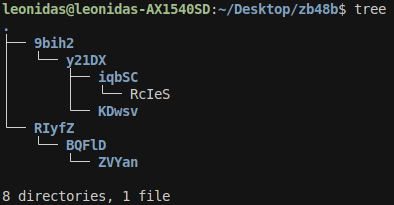
\includegraphics[width=0.95\textwidth]{images/image2.png}
  \caption{Дерево, воспроизведённое мной в терминале}
  \label{fig:my_tree}
\end{figure}






